%%Dokumentace k projektu soukrome knihovny na X33EJA
\documentclass{article}

\usepackage[utf8]{inputenc}
\usepackage{graphicx}
\usepackage[T1]{fontenc}
\usepackage{lmodern}
\usepackage[czech]{babel}
\usepackage{graphicx}
\usepackage{hyperref}


\title{Soukromá knihovna\\
 Semestrální projekt na předmět X33EJA}
\date{March 4, 2011}
\author{Petr Ondřejíček, Šimon Šťastný\\
FEL ČVUT v Praze}

\begin{document}

\begin{titlepage}
  \maketitle
  \thispagestyle{empty}
\end{titlepage}


\newpage

%------------------------------- Software Requirements Specification -----------
\part{Software Requirements Specification}

\vspace{10mm}
\smallskip

\indent \par Tento oddíl dokumentu popisuje stručne chování požadované od
systému a obsahuje též seznam funkčních požadavků na navrhovaný systém pro malou
osobní knihovnu. Uvedené popisy požadavků nejsou v této verzi dokumentu
definitivní a slouží pouze jako nástin pro budoucí popis požadavků. Detaily
jednotlivých požadavků bude v budoucnu doplněny podle potřeby. Jednotlivé
požadyvky jsou doplněny UML modely pro USE CASE (případy užití). Detailní
scénáře jednotlivých případů užití zatím nebyly konzultovány.


\newpage

\section{Celkový popis systému}
\indent \par Systém pro malou knihovnu bude používán v domácím prostředí pro
osobní účely. Jedná se v podstatě o evidenci knih a jejich vypůček známým a
kamarádům. Systém tedy nebude pracovat jako v klasické knihovně, bude značně
omezen na funkcích tak aby vyhovoval svému poslání a byl co možná
nejjednodušší, aby se uživatel netopil ve zbytečných funkcích, které v domácám
protředí nebudou použitelné.

\bigskip

Systém by měl v základu umožňovat evidenci čtenářů, tedy osob kterým budou moci
být knihy propůjčeny, evidenci autorů knih, evidenci knižních titulů a jejich
výtisků (dále je pro jednoduchost budeme nazývat svazky jak je v knihovním
prostředí zvykem). Pro potřeby třídění a úplnosti též zavedeme kategorie knih a
vydavatele.

\bigskip

Systém by též měl nějakým způsobem být schopen po definované době (výpůjční
lhůtě) odeslat čtenáři e-mailem upomínku, že zapoměl vrátit knihu. Mechanismus
spouštění a odesílání bude specifikován později, v této fázi projektu nejsme
schopni určit přesné technické řešení.

\newpage

\section{Požadavky na systém}
\subsection{Evidence čtenářů}

Systém bude administrátorovi umožňovat správu čtenářů. U čtenáře evidujeme jeho
jméno, příjmení a kontaktní e-mail.
U kontaktního e-mailu by bylo záhodno aby byla udržována aktuální adresa. Systém
by měl umožňovat zasílání upomínek na nevrácené knihy přímo čtenářům. Pokud bude
e-mailová adresa na čtenáře neaktuální, pochopitelně si upomínku nepřečte.

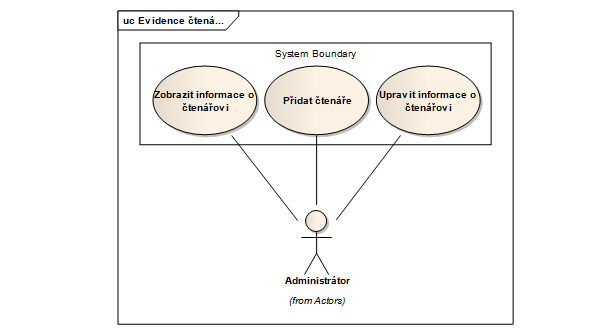
\includegraphics[width=350pt]{img/evidencectenaru.png}
\subsubsection{Přidat čtenáře}
Administrátor bude moci přidat do systému čtenáře.

\subsubsection{Zobrazit informace o čtenářovi}
Administrátor si bude moci zobrazit informace o čtenářovi, jeho komentáře k
titulům a historii jeho výpůjček.

\subsubsection{Upravit informace o čtenářovi}
Administrátor může změnit informace o čtenářovi.

\newpage
\subsection{Evidence svazků}
Systém bude administrátorovi umožňovat správu a půjčování svazků. U svazků
evidujeme titul, jeho je svazek výtiskem.

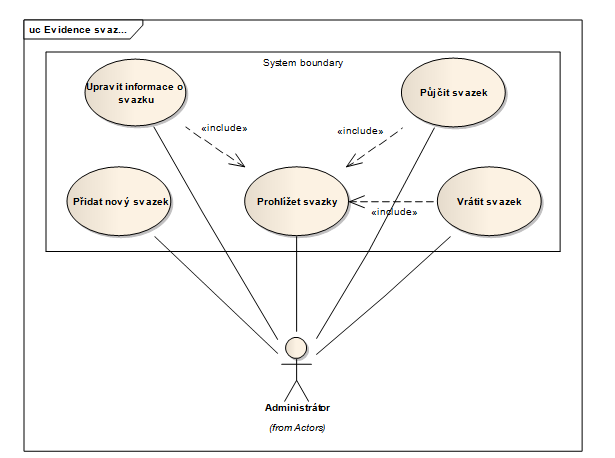
\includegraphics[width=350pt]{img/evidencesvazku.png}
\subsubsection{Přidat nový svazek}
Administrátor může přidat do systému nový svazek. Buďto k vybranému titulu, nebo
se odpovídající titul vytvoří.

\subsubsection{Prohlížet svazky}
Administrátor nebo čtenář si může prohlížet seznamy svazků.

\subsubsection{Upravit informace o svazku}
Administrátor může upravit informace o svazku.

\subsubsection{Půjčit svazek}
Administrátor může zaznamenat, že byl konkrétní svazek zapůjčen některému ze
čtenářů. Pokud je svazek zapůčen delší než definovanou výpůjční lhůtu, je
čtenáři zaslána e-mailová upomínka na kontaktní e-mailovou adresu.

\subsubsection{Vrátit svazek}
Administrátor může zaznamenat, že byl svazek čtenářem navrácen zpět do knihovny.


\subsection{Evidence autorů}
Systém bude administrátorovi umožňovat evidenci autorů. U autorů budeme evidovat
jejich jméno. Systém bude u autora též schopen zjistit jím napsané knihy v
systému.

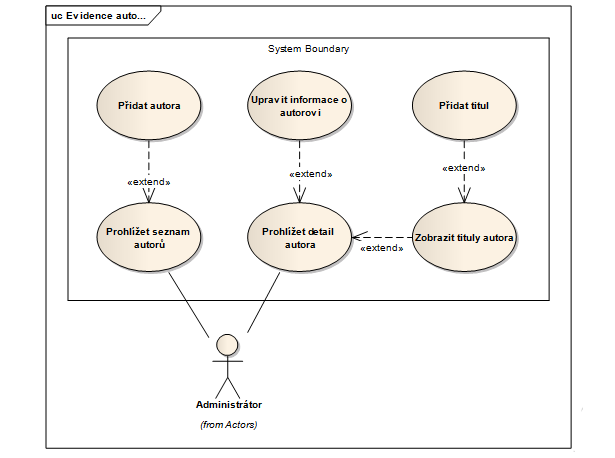
\includegraphics[width=350pt]{img/evidenceautoru.png}
\subsubsection{Přidat nového autora}
Administrátor může přidat do systému nového autora.

\subsubsection{Prohlížet autory}
Administrátor může prohlížet seznam autorů.

\subsubsection{Prohlížet detail autora}
Administrátor může prohlížet detail autora.

\subsubsection{Upravit informace o autorovi}
Administrátor může upravovat informace o autorovi.

\subsubsection{Zobrazit tituly autora}
Administrátor může prohlížet seznam titulů autora.

\subsection{Administrace knih}
Systém bude umožňovat správu knižních titulů. I titulu budeme evidovat jméno v
originále, kategorii knihy, ISBN, číslo vydání, vydavatele, autora, počet
stránek a stručný popis knihy.

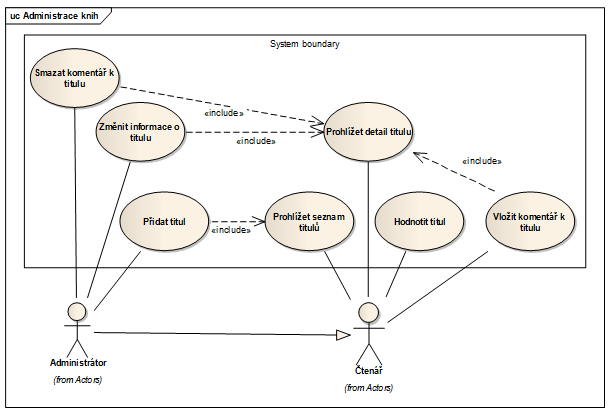
\includegraphics[width=350pt]{img/administraceknih.png}
\subsubsection{Přidat titul}
Administrátor může do systému přidat knižní titul.

\subsubsection{Prohlížet seznam titulů}
Administrátor nebo čtenář může prohlížet seznam titulů v databázi, řadit je dle
roku vydání, kategorie, autora, hodnocení.

\subsubsection{Prohlížet detail titulu}
Administrátor nebo čtenář může prohlížet detail titulu, budou zde zobrazeny výše
uvedené informace, komentáře uživatelů a níže popsané ohodnocení titulu.

\subsubsection{Upravit informace o titulu}
Administrátor může upravovat detail titulu.


\subsubsection{Hodnotit titul}
Systém bude umožňovat hodnocení titulu čtenáři. Čtenář bude mít možnost
ohodnotit knižní titul hodnocením od 0 do 10 bodů. Na detailu titulu se poté
bude zobrazovat průměřné hodnocení od všech čtenářů.

\subsubsection{Vložit komentář k titulu}
Administrátor nebo čtenář může vkládat komentář k titulu.

\subsubsection{Smazat komentář k titulu}
Administrátor může smazat libovolný komentář k titulu.

\subsection{Evidence kategorií}
Systém bude umožňovat správu kategorií, které se používají pro třídění knih.

\subsubsection{Přidat kategorii}
Administrátor může přidat kategorii.

\subsubsection{Smazat kategorii}
Administrátor může smazat kategorii.

\subsection{Evidence vydavatelů}
Systém bude umožňovat správu vydavatelů, které se používají pro třídění knih.

\subsubsection{Přidat vydavatele}
Administrátor může přidat vydavatele.

\subsubsection{Smazat vydavatele}
Administrátor může smazat vydavatele.



\newpage

\part{Datový model}

\vspace{10mm}
\smallskip

\indent \par Tento oddíl dokumentu popisuje vyhotovený datový model navrhovaného
systému. Součástí dokumentu je doménový slovník a ER model databáze.

\newpage

\section{Doménový slovník}

Vzhledem k tomu, že datový model je v anglickém jazyce, rozhodli jsme se jako
dodatek přiložit doménový slovník, který obsahuje v českém i anglickém jazyce
pojmy, kterými se model zabývá.

\begin{itemize}

\item Library Unit -- knihovní jednotka, svazek, výtisk

\item Book Title -- knižní titul

\item Charge Out -- absenční výpůjčka

\item Reader -- čtenář

\item Publisher -- vydavatel

\item Author -- autor

\item Category -- kategorie

\item Commentary -- komentář

\end{itemize}

\newpage


\section{Entity-Relationship Model}

Zde je zobrazen ER model navrhovaného systému.

\bigskip
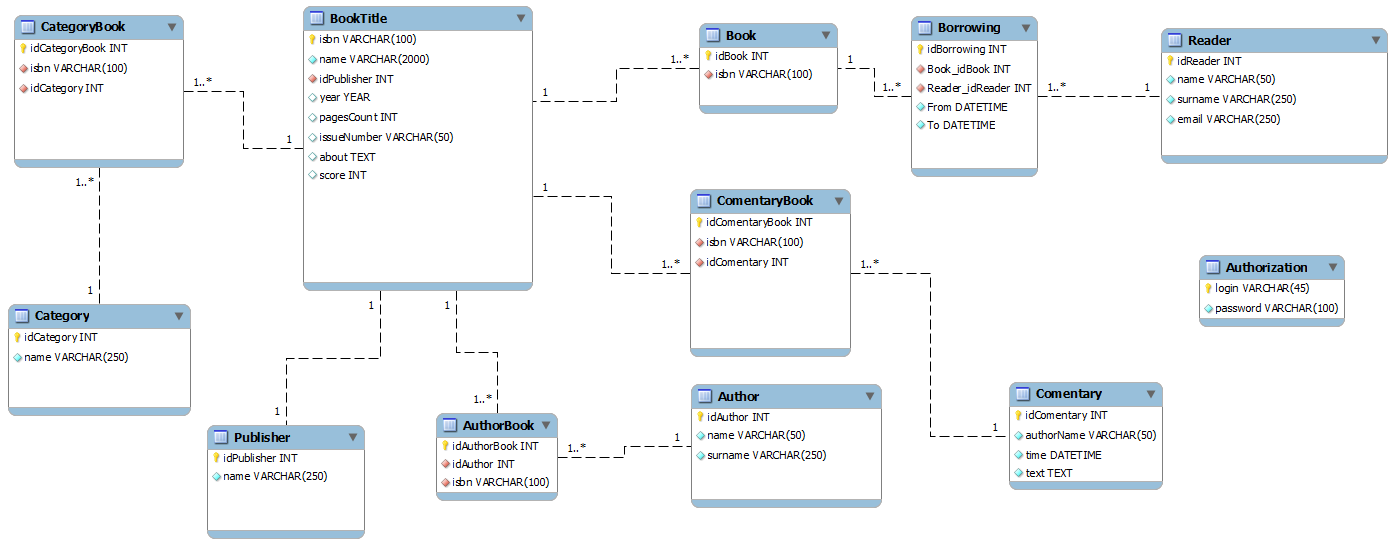
\includegraphics[width=450pt, angle=90]{img/ERM.png}

\newpage
\tableofcontents 

\end{document}
